
\documentclass [MS] {uclathes}

% \input {mymacros}                         % personal LaTeX macros

\usepackage[T1]{fontenc}
%\usepackage{tgbonum}
\usepackage{mathptmx}

\usepackage{pdfpages}

\setcounter{tocdepth}{4}
\setcounter{secnumdepth}{4}

\usepackage{xcolor}
\definecolor{uclablue}{HTML}{2774AE}
\usepackage{hyperref}
\hypersetup{
    colorlinks,
    citecolor=black,
    filecolor=black,
    linkcolor=uclablue,
    urlcolor=black
}

% https://tex.stackexchange.com/questions/75168/get-current-section-name-without-label
\usepackage{nameref}
\makeatletter
\newcommand*{\currentname}{\@currentlabelname}
\makeatother

\usepackage{chngcntr}
\counterwithout{section}{chapter}
\counterwithout{figure}{section}
\counterwithout{table}{section}
\counterwithin*{table}{section}

\setcounter{section}{-1}

\usepackage[explicit]{titlesec}
\newcommand*\Hide{%
\titleformat{\chapter}[display]
  {}{}{0pt}{\Huge}
\titleformat{\part}
  {}{}{0pt}{}
}

% https://tex.stackexchange.com/questions/458152/hidden-pages-in-latex
%\newcommand{\optional}[1]{#1}
\newcommand{\optional}[1]{}

%\renewcommand{\thetable}{S\arabic{table}}
%\renewcommand{\thetable}{\arabic{chapter}.S\arabic{table}}

% \newcommand\startsupplement{%
%     \makeatletter 
%       \setcounter{table}{0}
%       \renewcommand{\thetable}{S\arabic\c@table}
%     \makeatother}
    
% \newcommand{\hbAppendixPrefix}{S}
% %
% \renewcommand{\thefigure}{\hbAppendixPrefix\arabic{figure}}
% \setcounter{figure}{0}
% \renewcommand{\thetable}{\hbAppendixPrefix\arabic{table}} 
% \setcounter{table}{0}

%https://anneurai.net/2017/10/18/thesis-formatting-in-latex/
% \usepackage{epigraph}
% \setlength\epigraphwidth{1\textwidth}
% \setlength\epigraphrule{0pt} % no line between
% \setlength\beforeepigraphskip{1\baselineskip} % space before and after epigraph
% \setlength\afterepigraphskip{2\baselineskip}
% \renewcommand*{\textflush}{flushright}
% \renewcommand*{\epigraphsize}{\normalsize\itshape}

%https://hbfs.wordpress.com/2011/01/18/epigraphs-in-latex/
\newcommand\bookepigraph[4]{
\vspace{1em}\hfill{}\begin{minipage}{#1}{\begin{spacing}{0.9}
\small\noindent\textit{#2}\end{spacing}
\vspace{1em}
\hfill{}{#3}\\
 
\vspace{-1em}\begin{flushright}{#4}\end{flushright}}\vspace{2em}
\end{minipage}}

\newcommand\epigraph[3]{
\vspace{1em}\hfill{}\begin{minipage}{#1}{
\small\noindent\textit{#2}
\vspace{1em}
\hfill{}{#3}}\vspace{2em}
\end{minipage}}

% https://tex.stackexchange.com/questions/358766/exclude-chapter-from-toc-without-removing-numbering
\newcounter{oldtocdepth}

\newcommand{\hidefromtoc}{%
  \setcounter{oldtocdepth}{\value{tocdepth}}%
  \addtocontents{toc}{\protect\setcounter{tocdepth}{-10}}%
}

\newcommand{\unhidefromtoc}{%
  \addtocontents{toc}{\protect\setcounter{tocdepth}{\value{oldtocdepth}}}%
}

%%%%%%%%%%%%%%%%%%%%%%%%%%%%%%%%%%%%%%%%%%%%%%%%%%%%%%%%%%%%%%%%%%%%%%
%
% Usually things live in separate flies.
%
% \input {prelim}                           % preliminary page info

%%%%%%%%%%%%%%%%%%%%%%%%%%%%%%%%%%%%%%%%%%%%%%%%%%%%%%%%%%%%%%%%%%%%%%%%
%                                                                      %
%                          PRELIMINARY PAGES                           %
%                                                                      %
%%%%%%%%%%%%%%%%%%%%%%%%%%%%%%%%%%%%%%%%%%%%%%%%%%%%%%%%%%%%%%%%%%%%%%%%
%Rapid Automated High-Throughput Organismal Image Segmentation using Deep Learning for Analyses of Phenotypes at Massive Phylogenetic Scales
\title          {Automated High-Throughput Organismal \\
                Image Segmentation Using \\
                Deep Learning for \\ Massive Phenotypic Analysis}
\author         {Shawn Tyler Schwartz}
\department     {Biology}
% Note:  degreeyear should be optional, but as of  5-Feb-96
% it seems required or you get a year of ``2''.   -johnh
\degreeyear     {2021}

%%%%%%%%%%%%%%%%%%%%%%%%%%%%%%%%%%%%%%%%%%%%%%%%%%%%%%%%%%%%%%%%%%%%%%%%

\chair          {Michael Edward\ Alfaro}
\member         {Gregory Frank\ Grether}
\member         {Felipe Zapata}

%%%%%%%%%%%%%%%%%%%%%%%%%%%%%%%%%%%%%%%%%%%%%%%%%%%%%%%%%%%%%%%%%%%%%%%%

% \dedication     {\textsl{To my mother \ldots \\
%                 who---among so many other things--- \\
%                 saw to it that I learned to touch-type \\
%                 while I was still in elementary school}}

\dedication{\textsl{To Alma \ldots \\
who gave me the courage \\ --- and inspired me --- \\
to formally investigate \\ charismatic biodiversity}}
%%%%%%%%%%%%%%%%%%%%%%%%%%%%%%%%%%%%%%%%%%%%%%%%%%%%%%%%%%%%%%%%%%%%%%%%

\acknowledgments {I'd like to thank my advisor, Michael Alfaro, for taking me under his wing and teaching me the ropes of big data research. His support, feedback, and mentorship taught me how to be a critical scientist and ask questions that move the field forward. Prior to entering his lab --- first as an undergraduate research assistant in Fall 2018 prior to beginning my master's in Fall 2019 --- I lacked confidence in my ability to succeed as a scientist in academia. It was during Mike's \emph{Biology and Social Justice} (EE BIOL 156) seminar in the Summer of 2018 where we first met and I was captivated by the perspectives he put forth during our discussions. Mike made me think harder and deeper about the intersection of critical social issues with core biological concepts than I had ever done before. Had we not crossed paths then, I would have not had the opportunity to serve as the teaching assistant, and then associate, for EE BIOL 156 three times over during my master's --- one of my most fond memories of graduate school at UCLA. Mike, thank you for investing in me as an evolutionary biologist.

To my committee members, Greg Grether and Felipe Zapata, and additionally to my proposal reader, Nathan Kraft --- thank you all for your inspiration and guidance, especially in helping shape this research during its nascent stages.

To Alma, my lovely wife and best friend, for your tireless support, motivation, and inspiration --- especially when times were tough. I don't think I'd be where I am today had we not sat next to each other on the first day of our first-year neuroscience Fiat Lux seminar at UCLA in Spring 2016. Since then, you've taught me how to push the limits of what I thought was possible and to never give up when in the moments I was the weakest. From friendship and love to marriage, you've never once given up on me nor have you let me give up in the times I most wanted to --- I am forever grateful for this. During what seemed like a fun stay-at-home vacation at the beginning of the global COVID-19 pandemic in March of 2020 quickly turned out to be much scarier and less relaxing as we initially thought, but together we learned more about each other and began to cherish the fragility of life. I can't image spending those many months of isolation with anyone other than you and our Corgi puppy, Reese, who together form our beautiful and joyful family. Finally, you and Reese have taught me how to cope with my anxieties and other mental health issues --- especially during this pandemic --- and this immensely helped me keep my head up in the most challenging of times while completing the research presented in this thesis. I love you and can't thank you enough for helping shape me into a person I'm proud to be today.

I'd next like to thank my parents for their guidance and support during my childhood into adulthood. Specifically, thank you to my mom, Terri, for never hesitating to stay up late with me while I completed my homework or taking me around town when I needed a lift to school or the science fair. To my dad, Bruce, for making time to spend with us despite working on-call, 24/7 in a blue-collar profession. I would not be the person I am today without their love and care. I'd also like to thank my sister, Nicole, for encouraging me to get up from the computer and play outside every once and a while when we were kids. Her artistic creativity has been a source of inspiration for me in the times I've lacked creativity myself. I'd also like to thank my brother and sister in-laws, Rafael and Laura, for always being available to give advice and make me laugh with a joke or funny video when I've needed it most. Rafael, as we've embarked on our graduate school journey together, I'm so excited and enthusiastic to see where our careers take us, and I couldn't have asked for a better brother, and friend, to grow professionally with as first-generation students in academia. Por último, a mis suegros, Teresa y Rafael, por inspirarme a aprender español, apreciar la vida y disfrutar de las hermosas y ricas comidas de Chavinda, Michoacán, México.

Next, to those who were instrumental in my pedagogical growth as an instructor, especially the UCLA Center for the Integration of Research, Teaching, and Learning (CIRTL@UCLA) and the UCLA Center for Education Innovation \& Learning in the Sciences (CEILS). I'd specifically like to thank Rachel Kennison, Leigh Harris, Katie Dixie, and Elizabeth Reid-Wainscoat for their support and mentorship, in addition to the UCLA CIRTL Teaching-as-Research (TAR) community, especially Manisha Chase, Shawn McEachin, Annie Wofford, Amelia Hill, Letty Treviño, and Chelsea Romney for their support and engagement during the sudden shift to remote instruction at the onset of the COVID-19 pandemic --- thank you \emph{CIRTL turtles} for always being such a welcoming and positive community! To my other instructional mentors --- Michael Alfaro, Pamela Yeh, Rachel Prunier, Iris Firstenberg, Amber Ankowski, Elizabeth Bjork, Alan Castel, Tyler McCraney, Ginny Sklar, Manisha Chase, and Mary Whatley  --- for showing me the importance of compassion and flexibility through your passion for teaching and care for students; you've all played a role in shaping me as the teacher I am today.

Lastly, I'd like to thank all of those who --- directly and indirectly --- contributed to the research presented in this thesis. To Elizabeth Karan, Whitney Nakashima, and Mark Juhn, for many insightful and inspirational conversations about color pattern diversity, mechanisms, and deep learning to helping me find my way when hitting programming walls. I'm grateful for our friendship born out of the many in-person discussions prior to the pandemic, in addition to the fun virtual social gatherings on Zoom that made doing science while sheltering in place less isolating. To Tyler McCraney, for always making me feel welcome and for useful advice about how to ask interesting and fun scientific questions that excite and motivate me. To Christiane Jacquemetton and Jonathan Chang, for helpful grad school, professional, and life advice that I'll take with me to each stage of my professional career. To Alex Siegel, for being an awesome friend and collaborator, and for being instrumental in teaching me more advanced statistical modeling methods and leading me to find my true research passions studying the neuroscience of memory and cognitive aging. To Alan Castel, for your mentorship and guidance in research, especially in helping me conduct my first independent research study during undergrad and guiding me to where I am today as a professional in academia. To my many collaborators and coauthors --- both past and present --- especially, Allison Shultz, Lars Schmitz, Katie Silaj, Mary Whatley, Dillon Murphy, Hannah Weller, Mary Hargis, Lauren Richmond, Julia Kearley, Ian McDonough, and Neil Garg. To the wonderful research assistants who've been instrumental in getting some of this (and other) research off the ground and for reminding me of the joy and inspiration that comes with mentorship: Mackenzie Perillo, Maya Chari, Aubrey Butler, Kevin Wang, Jonathan Chau, Nimrat Brar, Trevor Brokowski, Kate Javerbaum, Austyn Adams, Kyle Xu, and Charles Wang.

The work presented in this thesis is a reprint of: Shawn T. Schwartz, \& Michael E. Alfaro (2021). \emph{Sashimi}: A toolkit for facilitating high-throughput organismal image segmentation using deep learning. \textit{Methods in Ecology and Evolution, 12}, 2341–2354. \href{https://doi.org/10.1111/2041-210X.13712}{doi:10.1111/2041-210X.13712}. S.T.S. and M.E.A. conceived of the study; S.T.S. wrote the software. Both authors contributed to the writing of the manuscript.}


%%%%%%%%%%%%%%%%%%%%%%%%%%%%%%%%%%%%%%%%%%%%%%%%%%%%%%%%%%%%%%%%%%%%%%%%

\epigraphpage{
%\bookepigraph{2in}{This is a most excellent epigraph macro for
%\LaTeX.}{some name}{from Some Book}
\epigraph{5in}{There’s lots of ways to be as a person, and some people express their deep appreciation in different ways, but one of the ways that I believe people express their appreciation to the rest of humanity is to make something wonderful and put it out there. And you never meet the people, you never shake their hands, you never hear their story or tell yours, but somehow, in the act of making something with a great deal of care and love, something is transmitted there. And it’s a way of expressing to the rest of our species our deep appreciation. So, we need to be true to who we are and remember what’s really important to us.}{--- \fauxsc{Steve Jobs}}
 
}
% \epigraphpage{
%     \epigraph{``There’s lots of ways to be as a person, and some people express their deep appreciation in different ways, but one of the ways that I believe people express their appreciation to the rest of humanity is to make something wonderful and put it out there. And you never meet the people, you never shake their hands, you never hear their story or tell yours, but somehow, in the act of making something with a great deal of care and love, something is transmitted there. And it’s a way of expressing to the rest of our species our deep appreciation. So, we need to be true to who we are and remember what’s really important to us.''}{--- \fauxsc{Steve Jobs}, \small\textup{Co-Founder and Former CEO of Apple Inc.}}

% }
%\epigraphpage {\epigraph{``There’s lots of ways to be as a person, and some people express their deep appreciation in different ways, but one of the ways that I believe people express their appreciation to the rest of humanity is to make something wonderful and put it out there. And you never meet the people, you never shake their hands, you never hear their story or tell yours, but somehow, in the act of making something with a great deal of care and love, something is transmitted there. And it’s a way of expressing to the rest of our species our deep appreciation. So, we need to be true to who we are and remember what’s really important to us.''}{--- Steve Jobs, \emph{Co-Founder and Former CEO of Apple Inc.}}}

%%%%%%%%%%%%%%%%%%%%%%%%%%%%%%%%%%%%%%%%%%%%%%%%%%%%%%%%%%%%%%%%%%%%%%%%

\abstract       {Utilizing the comparative method at massive analytic scales requires the acquisition of large samples of characters for taxa across the tree of life. When data acquisition approaches are limited, studies may subsequently limit their analysis to a particularly conserved group of taxa to avoid issues of incomplete sampling at larger phylogenetic scales. The inherent difficulty associated with obtaining large datasets imposes a data bottleneck for studying comparative macroevolution through deep time scales. Having access to powerful and flexible artificially intelligent approaches for data acquisition and pre-processing are therefore important for facilitating larger scales of analysis. Machine learning provides unprecedented opportunities to exploit massive datasets. The subsequent development of deep learning applications specialized for automating cumbersome human tasks is possible given that these models learn over time to perform such tasks with accuracy similar to that of a human observer. Deep learning is a branch of machine learning that holds enormous potential for ecologists and evolutionary biologists in an era of research becoming increasingly reliant on big data. These tools can streamline data extraction from field observations and recordings, in addition to uncovering complex patterns in dense multivariate datasets. Here, I focus on leveraging deep learning as a toolkit for image segmentation. This toolkit,  \emph{Sashimi}, provides a reproducible, rapid, and automated approach for pre-processing digitized images of organisms necessary for downstream analyses of visual phenotypes --- such as color patterns --- at massive phylogenetic scales.}

%%%%%%%%%%%%%%%%%%%%%%%%%%%%%%%%%%%%%%%%%%%%%%%%%%%%%%%%%%%%%%%%%%%%%%%%

%%%%%%%%%%%%%%%%%%%%%%%%%%%%%%%%%%%%%%%%%%%%%%%%%%%%%%%%%%%%%%%%%%%%%%%%

\begin{document}
\makeintropages

% \hidefromtoc
% \chapter*{Epigraph}
% \unhidefromtoc
%https://www.goodreads.com/quotes/8785521-there-s-lots-of-ways-to-be-as-a-person-and
%\epigraph{``There’s lots of ways to be as a person, and some people express their deep appreciation in different ways, but one of the ways that I believe people express their appreciation to the rest of humanity is to make something wonderful and put it out there. And you never meet the people, you never shake their hands, you never hear their story or tell yours, but somehow, in the act of making something with a great deal of care and love, something is transmitted there. And it’s a way of expressing to the rest of our species our deep appreciation. So, we need to be true to who we are and remember what’s really important to us.''}{--- Steve Jobs, \emph{Co-Founder and Former CEO of Apple Inc.}}

%%%%%%%%%%%%%%%%%%%%%%%%%%%%%%%%%%%%%%%%%%%%%%%%%%%%%%%%%%%%%%%%%%%%%%
%
% Ordinarily each chapter (at least) is in a separate file.
%
%% https://tex.stackexchange.com/questions/458152/hidden-pages-in-latex
\optional{
%\Hide
% https://tex.stackexchange.com/questions/228729/how-to-hide-chapter-numbering-in-table-of-contents
\chapter*{\emph{Sashimi}: A toolkit for facilitating high-throughput organismal image segmentation using deep learning}
\addcontentsline{toc}{chapter}{\emph{Sashimi}: A toolkit for facilitating high-throughput organismal image segmentation using deep learning}
}

\clearpage

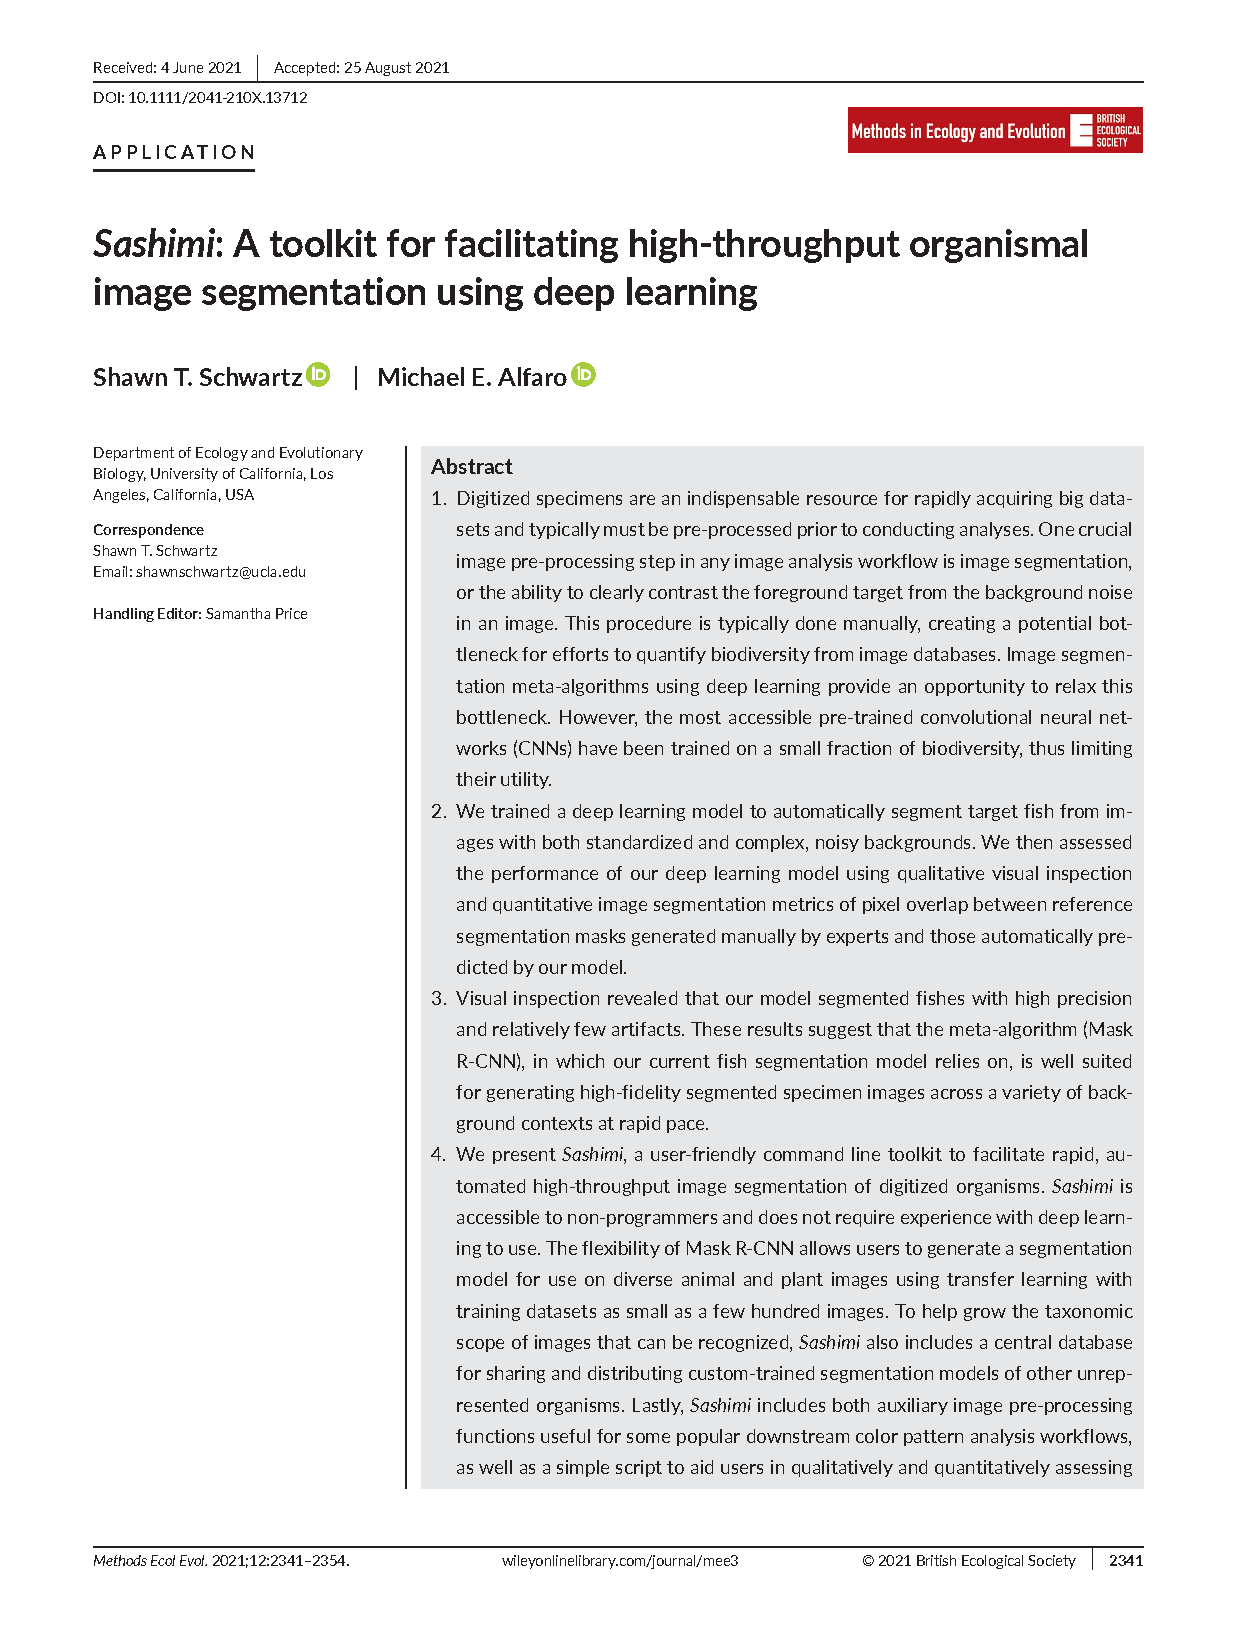
\includepdf[scale=0.85, pages=1-14, pagecommand={}, addtotoc={
     1,section,1,Abstract,abstract,
     2,section,1,Introduction,intro,
     4,section,1,Materials and Methods,materialsandmethod,
     4,subsection,1,Mask R-CNN architecture,architecture,
     4,subsection,1,Model training dataset acquisition,dataset,
     4,subsection,1,Model training procedure,training,
     4,subsection,1,Automated segmentation pipeline,pipeline,
     4,subsection,1,\emph{Sashimi} online model repository,repo,
     4,subsection,1,Evaluating fish segmentation model efficacy,modeleval,
     4,subsubsection,2,Qualitative image segmentation evaluation,qualseg,
     5,subsubsection,2,Quantitative image segmentation evaluation metrics,quantseg,
     7,subsection,1,Statistics,stats,
     7,section,1,Results,results,
     7,subsection,1,Qualitative image segmentation evaluation,qualsegres,
     8,subsection,1,Quantitative image segmentation evaluation metrics,quantsegres,
     9,section,1,Discussion,discussion,
     11,section,1,Acknowledgements,acks,
     11,section,1,Conflict of Interest,interest,
     11,section,1,Authors' Contributions,contrib,
     12,section,1,Peer Review,peerrev,
     12,section,1,Data Availability Statement,openscience,
     12,section,1,ORCID,orcid,
     12,section,1,References,refs
     }, addtolist={5,figure,Examples of diverse fish images used for model training,fig1,
     6,figure,Examples of predicted segmentation masks generated by custom-trained fish segmentation model,fig2,
     7,figure,Examples of fish images automatically segmented by \emph{Sashimi},fig3,
     8,figure,Butterflyfishes segmented by humans along with naïve and custom-trained COCO models,fig4,
     9,figure,(a) \emph{Forcipiger} Butterflyfishes segmented by humans and \emph{Sashimi}; (b) Automatically segmented fishes with stray pixels,fig5,
     10,figure,Segmentation of novel fish images in natural noisy contexts,fig6,
     11,figure,Image segmentation evaluation metrics,fig7,
     11,table,Post hoc comparisons for the main effect of evaluation metric,tab1
     }]{pdfs/sashimi_mee_main.pdf}
    %  \startsupplement
    
    % https://tex.stackexchange.com/questions/104479/table-numbering-style/104484
    % https://tex.stackexchange.com/questions/85776/change-figure-numbering-for-appendix
    \appendix
    \counterwithin{table}{section}
    \renewcommand{\thesection}{S\arabic{section}}
    \renewcommand{\thetable}{S\arabic{table}}
\includepdf[scale=1, pages=1-78, pagecommand={}, addtotoc={
1,section,1,Supporting Information,suppinfo,
4,subsection,1,Quantitative image segmentation evaluation metrics for novel test set,quantimgevalnovel,
8,subsection,1,Color pattern analysis comparison,colorpatternanalysis,
10,subsection,1,Results,suppres,
14,subsection,1,iNaturalist novel test set (\textit{n} = 30) visual evaluations,inatvizeval,
45,subsection,1,J.E. Randall novel test set (\textit{n} = 30) visual evaluations,randallvizeval,
76,subsection,1,References,supprefs}, addtolist={1,table,Post hoc comparisons for the interaction between accuracy metric and image source (validation set),s1,
5,table,Post hoc comparisons for the main effect of evaluation metric (test set),s2,
6,table,Post hoc comparisons for the interaction between accuracy metric and image source (test set),s3,
11,table,MANOVA,s4,
13,table,Descriptive statistics for color pattern geometry variables,s5}]{pdfs/sashimi_mee_supp.pdf}                         % Chapter 1 of dissertation
%\input {chapter2}                         % Chapter 2
%\input {chapter3}                         % etc.
%\input {chapter4}
%\input {chapter5}
%\input {chapter6}
%\input {chapter7}
%\input {chapter8}



% https://tex.stackexchange.com/questions/458152/hidden-pages-in-latex
\optional{
%\Hide
% https://tex.stackexchange.com/questions/228729/how-to-hide-chapter-numbering-in-table-of-contents
\chapter*{\emph{Sashimi}: A toolkit for facilitating high-throughput organismal image segmentation using deep learning}
\addcontentsline{toc}{chapter}{\emph{Sashimi}: A toolkit for facilitating high-throughput organismal image segmentation using deep learning}
}

\clearpage

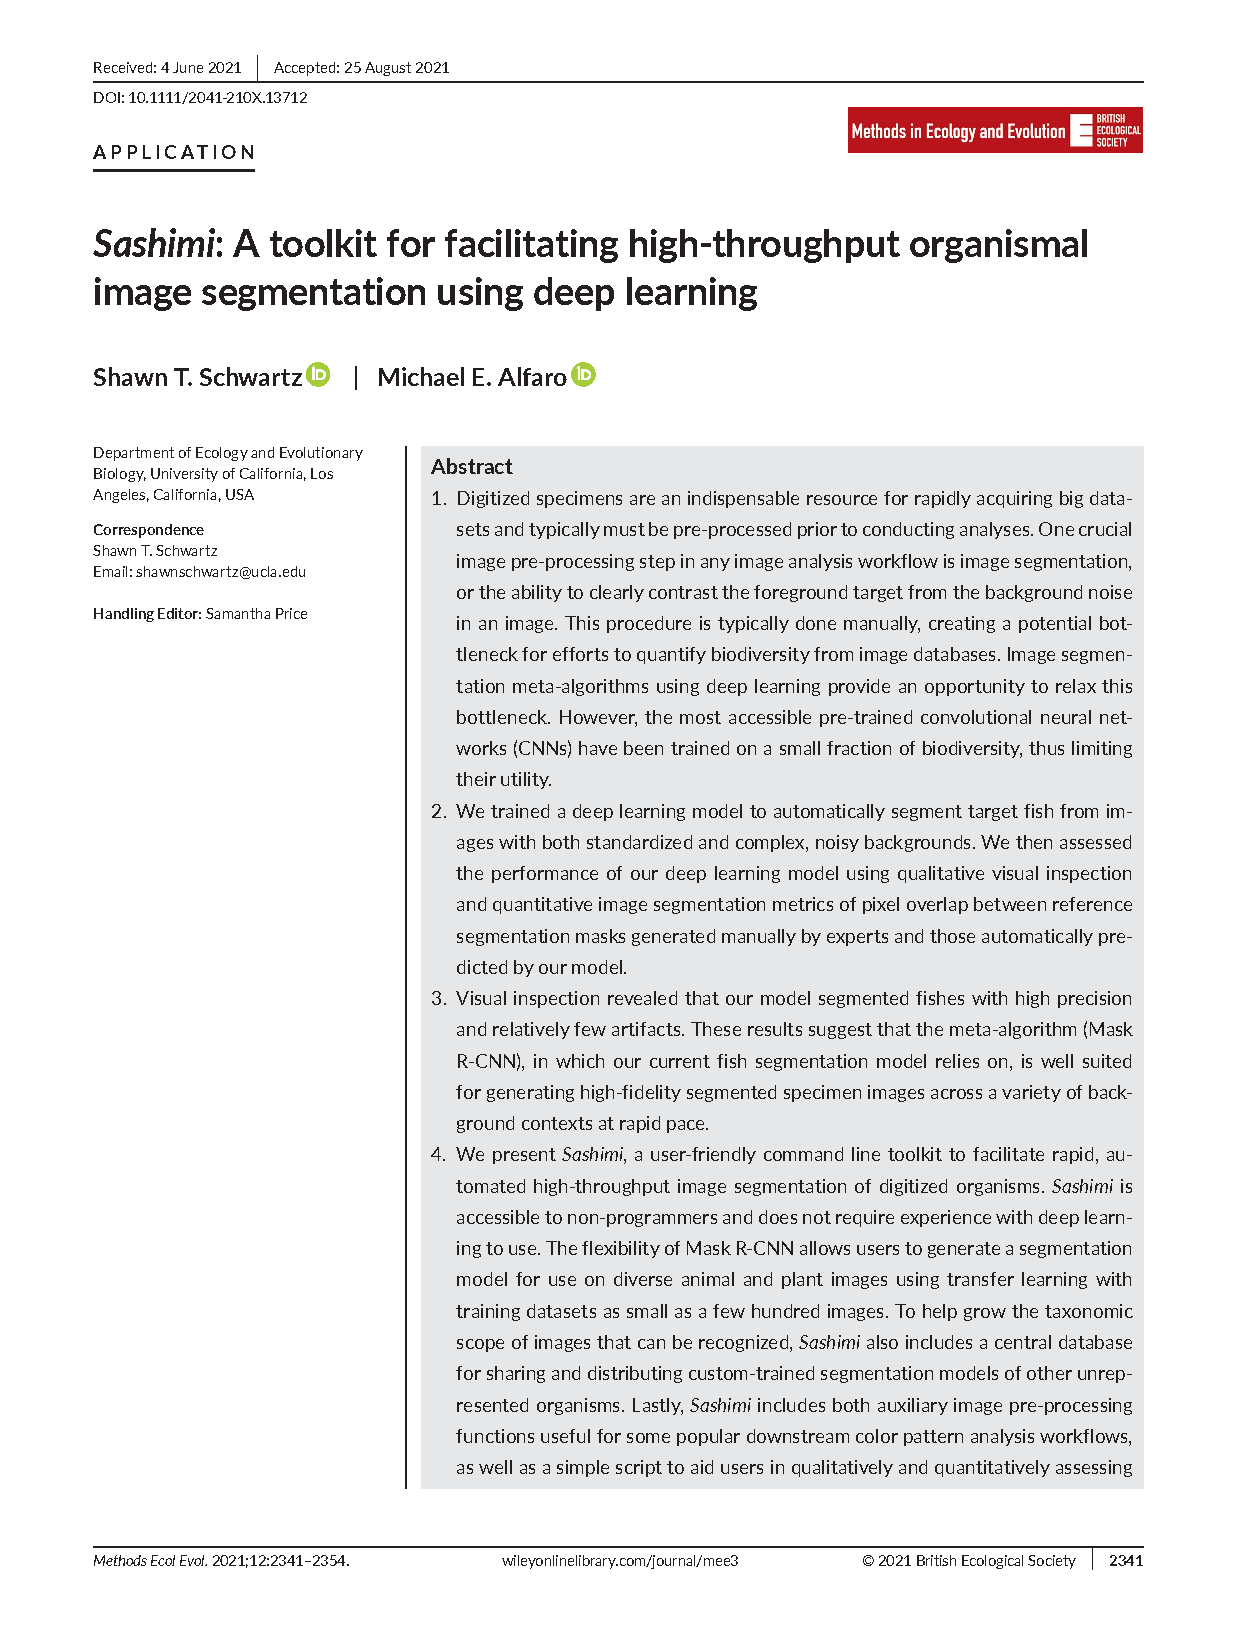
\includepdf[scale=0.85, pages=1-14, pagecommand={}, addtotoc={
     1,section,1,Abstract,abstract,
     2,section,1,Introduction,intro,
     4,section,1,Materials and Methods,materialsandmethod,
     4,subsection,1,Mask R-CNN architecture,architecture,
     4,subsection,1,Model training dataset acquisition,dataset,
     4,subsection,1,Model training procedure,training,
     4,subsection,1,Automated segmentation pipeline,pipeline,
     4,subsection,1,\emph{Sashimi} online model repository,repo,
     4,subsection,1,Evaluating fish segmentation model efficacy,modeleval,
     4,subsubsection,2,Qualitative image segmentation evaluation,qualseg,
     5,subsubsection,2,Quantitative image segmentation evaluation metrics,quantseg,
     7,subsection,1,Statistics,stats,
     7,section,1,Results,results,
     7,subsection,1,Qualitative image segmentation evaluation,qualsegres,
     8,subsection,1,Quantitative image segmentation evaluation metrics,quantsegres,
     9,section,1,Discussion,discussion,
     11,section,1,Acknowledgements,acks,
     11,section,1,Conflict of Interest,interest,
     11,section,1,Authors' Contributions,contrib,
     12,section,1,Peer Review,peerrev,
     12,section,1,Data Availability Statement,openscience,
     12,section,1,ORCID,orcid,
     12,section,1,References,refs
     }, addtolist={5,figure,Examples of diverse fish images used for model training,fig1,
     6,figure,Examples of predicted segmentation masks generated by custom-trained fish segmentation model,fig2,
     7,figure,Examples of fish images automatically segmented by \emph{Sashimi},fig3,
     8,figure,Butterflyfishes segmented by humans along with naïve and custom-trained COCO models,fig4,
     9,figure,(a) \emph{Forcipiger} Butterflyfishes segmented by humans and \emph{Sashimi}; (b) Automatically segmented fishes with stray pixels,fig5,
     10,figure,Segmentation of novel fish images in natural noisy contexts,fig6,
     11,figure,Image segmentation evaluation metrics,fig7,
     11,table,Post hoc comparisons for the main effect of evaluation metric,tab1
     }]{pdfs/mee_main.pdf}
    %  \startsupplement
    
    % https://tex.stackexchange.com/questions/104479/table-numbering-style/104484
    % https://tex.stackexchange.com/questions/85776/change-figure-numbering-for-appendix
    \appendix
    \counterwithin{table}{section}
    \renewcommand{\thesection}{S\arabic{section}}
    \renewcommand{\thetable}{S\arabic{table}}
\includepdf[scale=1, pages=1-78, pagecommand={}, addtotoc={
1,section,1,Supporting Information,suppinfo,
4,subsection,1,Quantitative image segmentation evaluation metrics for novel test set,quantimgevalnovel,
8,subsection,1,Color pattern analysis comparison,colorpatternanalysis,
10,subsection,1,Results,suppres,
14,subsection,1,iNaturalist novel test set (\textit{n} = 30) visual evaluations,inatvizeval,
45,subsection,1,J.E. Randall novel test set (\textit{n} = 30) visual evaluations,randallvizeval,
76,subsection,1,References,supprefs}, addtolist={1,table,Post hoc comparisons for the interaction between accuracy metric and image source (validation set),s1,
5,table,Post hoc comparisons for the main effect of evaluation metric (test set),s2,
6,table,Post hoc comparisons for the interaction between accuracy metric and image source (test set),s3,
11,table,MANOVA,s4,
13,table,Descriptive statistics for color pattern geometry variables,s5}]{pdfs/mee_supp.pdf}
\end{document}
%\bibliography {bib/network,bib/naming}    % bibliography references
%\bibliographystyle {thesis}



